\chapter{Teori}\label{Teori}

\section{A* Algoritmen}\label{A-Algoritmen}
Primært når det kommer til belægning af en dynamisk rute, foregår det ved at en enhed fortsætter hen i mod et mål indtil den når en forhindring. Dette er et ekstremt simpelt bevægelsesmønster og indebærer in vis in-effektivitet. Rent retorisk kunne man stille spørgsmålet om det ikke ville være smartere at planlægge en rute før man overhovedet bevæger sig.

A* er en algoritme til at beregne den korteste rute baseret på en række heuristiske datasæt. A* får input igennem en brugerlavet graf der indeholder en række datasæt for at algoritmen kan fungere.  Først har vi distancen fra punkt til punkt, eksempelvis punkt 'A' til punkt 'B' som vi kalder for f.eks. \textbf{'H'} og dernæst har vi et datasæt \textbf{'G'} der indeholder bekostningen for at flytte fra en kant til en anden, denne variabel er bestemt på forhånd. Et virkelighedseksempel kunne være at man vil over på den anden side af en sø, så har man så muligheden for at svømme direkte eller gå uden om og det koster f.eks. 2 gange så meget at bevæge sig direkte igennem søen. Dette er givet ved \textbf{'G'}, hvor som sagt \textbf{'H'} er den ultimative korteste længde til det bestemte slutpunkt. \textbf{'H'} fungerer desuden for hvilket som helst punkt i et system og angiver \textit{altid} den korteste vej til slutpunktet uanset forhindringer.

En måde man kan visualisere A* på er f.eks. med et gitter-system som set i figur \ref{A*Kvadrat-1}. Her kan vi se at vi har et start punkt (grøn) og et slutpunkts (blå). De gitre vi ikke kan bevæge os igennem er de røde firkanter. Figuren angiver ingen heuristiske datasæt endnu.

\begin{wrapfigure}{l}{0.60\textwidth}
    \centering
    \includegraphics[width=0.60\textwidth]{Pictures/Teoriafsnit/Figurfiler/Grid2.png}
    \caption{Kvadrat-system}
    \label{A*Kvadrat-1}
\end{wrapfigure}

Ud fra figuren kan vi begynde os at forestille hvordan A* fungerer. Når man bevæger sig fra firkant til firkant laver man 2 lister til at holde styr på hvor brikken har været. En liste til at holde styr på hvilke gitre man ikke har besøgt endnu og en liste der holder styr på hvilke man \textbf{'har'} besøgt. Når man flytter brikken skal man derfor angive hvilken firkant der nu skal på \textit{'besøgt'} listen. Derfor som nævnt skal vi bruge information om hvor meget \textbf{'G'} koster. Brikken skal nu til at flytte sig for at komme til slutpunktet. Dette kunne f.eks. være 1 point for at flytte sig i hvilken som helst retning, men man kunne også sagtens angive at diagonal bevægelse ville koste 4 point. Dvs. at ruten ændrer sig til måske ikke at være så direkte som den ellers kunne have været.

Der findes flere metoder man kan anvende A* på og en af dem vises her.
Det vises her i den lille bid af pseudo-kode i figur \ref{lst:A*pseudo1}
\begin{lstlisting}[caption={Pseudo-kode af lister i A*},label={lst:A*pseudo1}]
	class A_Star
	{
		List<int> nodeIdentifierVisited = new List<int> { 7, 8, 9 , 10, 11, 12, 13, 14, 21, 23, 24, 28, 29, 30, 31, 32};

		Expand to new node from previous and move
		Queue frontQueue = new Point();

		when Point is acknowledged to move
		change new Point to become Visited = true;

		while(new Point == Visited)
		{
			move Point to nodeIdentifierVisited
		}
	}
\end{lstlisting}